%% ============================================================
%%  LoanEase -- IEEE Conference Paper
%%  Authors: Agniv Dutta, Aditya Choudhuri, Akshat Kunder,
%%           Aaryan Dubey
%%  Institution: K.J. Somaiya College of Engineering,
%%               Somaiya Vidyavihar University, Mumbai
%%  Guide: Dr. Mansi Kambli
%% ============================================================

\documentclass[conference]{IEEEtran}

% ---- Core packages ----
\usepackage[T1]{fontenc}
\usepackage[utf8]{inputenc}
\usepackage{cite}
\usepackage{amsmath,amssymb,amsfonts}
\usepackage{algorithmic}
\usepackage{graphicx}
\usepackage{textcomp}
\usepackage{xcolor}
\usepackage{booktabs}
\usepackage{multirow}
\usepackage{array}
\usepackage{url}
\usepackage{hyperref}
\usepackage{microtype}
\usepackage{float}          % [H] hard float placement
\usepackage{placeins}       % \FloatBarrier

% ---- TikZ for diagrams ----
\usepackage{tikz}
\usetikzlibrary{
  shapes.geometric,
  arrows.meta,
  positioning,
  fit,
  backgrounds,
  calc,
  decorations.pathreplacing,
  shadows.blur
}

% ---- Listings for code snippets ----
\usepackage{listings}
\lstset{
  basicstyle=\ttfamily\scriptsize,
  breaklines=true,
  frame=single,
  backgroundcolor=\color{gray!8},
  keywordstyle=\color{blue!70},
  commentstyle=\color{green!50!black},
  stringstyle=\color{red!60!black},
  numbers=left,
  numberstyle=\tiny\color{gray},
  xleftmargin=1.5em
}

% ---- Color palette ----
\definecolor{loanBlue}{RGB}{20,74,140}
\definecolor{loanGold}{RGB}{201,150,0}
\definecolor{loanGreen}{RGB}{0,128,96}
\definecolor{loanRed}{RGB}{180,30,30}
\definecolor{loanGray}{RGB}{100,100,110}
\definecolor{loanLightBlue}{RGB}{220,236,255}
\definecolor{loanLightGold}{RGB}{255,248,220}
\definecolor{loanLightGreen}{RGB}{220,255,240}
\definecolor{loanLightRed}{RGB}{255,220,220}
\definecolor{agentBg}{RGB}{245,248,255}

% Rupee symbol workaround
\newcommand{\rupee}{\textrm{Rs.}}

% ---- Hyperref config ----
\hypersetup{
  colorlinks=true,
  linkcolor=loanBlue,
  citecolor=loanBlue,
  urlcolor=loanBlue
}

% ---- IEEEtran column sep tweak ----
\IEEEoverridecommandlockouts

% ============================================================
\begin{document}
% ============================================================


\title{LoanEase: A Multi-Agent AI Framework for Automated
Personal Loan Acquisition with Explainable Credit Risk
Assessment and Blockchain Auditability}

\author{
  \IEEEauthorblockN{
    Agniv Dutta,\;
    Aditya Choudhuri,\;
    Akshat Kunder,\;
    Aaryan Dubey
  }
  \IEEEauthorblockA{
    Department of Computer Engineering,\\
    K.J.\ Somaiya College of Engineering,
    Somaiya Vidyavihar University, Mumbai, India\\
    \{agniv.dutta, aditya.choudhuri, akshat.kunder,
      aaryan.dubey\}@somaiya.edu
  }
  \IEEEauthorblockN{\vspace{4pt}Guide: Dr.\ Mansi Kambli}
  \IEEEauthorblockA{
    Department of Computer Engineering,\\
    K.J.\ Somaiya College of Engineering,
    Somaiya Vidyavihar University, Mumbai, India
  }
}

\maketitle

% ============================================================
%  ABSTRACT
% ============================================================
\begin{abstract}
The personal loan acquisition process in India remains
predominantly manual, opaque, and time-consuming,
typically requiring 7--10 business days for approval
and relying on static paper forms with no real-time
applicant guidance. This paper presents \textbf{LoanEase},
a novel multi-agent AI framework that automates the
end-to-end personal loan lifecycle through five
collaborating specialized agents orchestrated by a
central large language model. The system integrates
OCR-based Know Your Customer (KYC) verification using
RapidOCR, an XGBoost credit underwriting classifier
augmented with SHAP explainability, a rule-based
multi-round loan negotiation engine, Groq LLaMA 3.3 70B
for multilingual Hindi/English/Hinglish conversational
support, and a SHA-256 blockchain audit trail for
tamper-proof sanction letter generation. Each agent
operates as an independent FastAPI microservice,
enabling horizontal scalability and fault isolation.
Evaluated on the Kaggle Loan Prediction Dataset (614
samples, 12 features), the XGBoost model achieves
82.1\% accuracy with an AUC-ROC of 0.87. LoanEase
demonstrates a \textbf{99.4\% reduction} in average
loan processing time---from 7--10 days to under 5
minutes---over traditional branch-based banking methods,
while providing transparent, explainable, and auditable
credit decisions.
\end{abstract}

\begin{IEEEkeywords}
Agentic AI, Multi-Agent Systems, Credit Risk Assessment,
XGBoost, SHAP Explainability, Large Language Models,
Blockchain Auditability, KYC Verification, Loan Processing,
Multilingual NLP
\end{IEEEkeywords}


% ============================================================
%  I. INTRODUCTION
% ============================================================
\section{Introduction}

India's formal credit market services approximately
190~million active borrowers, yet the Reserve Bank of
India (RBI) estimates that nearly 300~million credit-worthy
individuals remain unserved by traditional banking channels
\cite{rbi2024}. The conventional personal loan application
process demands physical branch visits, manual document
submission, static eligibility forms, and underwriter
queues that routinely extend over 7--10 business
days~\cite{niti2023digitalfinance}. Digital banking
portals have partially addressed accessibility, yet most
reduce processing to 2--3 days while still relying on
rule-based eligibility screens, offering no interactive
guidance, negotiation capability, or explanatory feedback
to rejected applicants.

The advent of Agentic AI---autonomous systems that can
plan, reason, and execute multi-step tasks---presents a
transformative opportunity for financial services
automation. Unlike single monolithic models, multi-agent
architectures decompose complex workflows into specialized
cognitive units that collaborate via defined communication
protocols \cite{wu2023autogen,wang2024survey}. Each agent
encapsulates domain expertise, enabling the system to
simultaneously handle document intelligence, risk
quantification, conversational negotiation, and regulatory
compliance within a unified orchestration loop.

Existing fintech chatbots address customer support but
rarely extend to full loan lifecycle automation. They
typically lack: (i) real-time OCR-based document
verification; (ii) model-explainable credit decisions;
(iii) dynamic multi-round interest rate negotiation bounded
by business policy; and (iv) cryptographically auditable
sanction letters. LoanEase addresses all four gaps within
a single agentic conversational interface.

The key contributions of this paper are:
\begin{itemize}
  \item A five-agent architecture for complete personal
        loan automation from KYC to sanction letter.
  \item A combined credit scoring formula blending
        deterministic CIBIL simulation with XGBoost
        probability under a 60/40 weighting scheme.
  \item SHAP-based plain-English underwriting explanations
        that improve decision transparency.
  \item A stateful multi-round negotiation engine with
        risk-tier-aware concession policies.
  \item Blockchain-anchored sanction letters via SHA-256
        hashing with Ethereum-compatible structure.
\end{itemize}

The remainder of this paper is organized as follows.
Section~II surveys related work across agentic AI
frameworks, credit risk modeling, and blockchain in
finance. Section~III presents the overall system
architecture. Section~IV details the methodology for
each subsystem. Section~V reports experimental results.
Section~VI discusses implications and limitations.
Section~VII concludes with future research directions.

% ============================================================
%  II. RELATED WORK
% ============================================================
\section{Related Work}

\subsection{Agentic AI Frameworks}

Wu~et~al.\ \cite{wu2023autogen} introduced \textit{AutoGen},
a framework enabling multi-agent conversations among
LLM-powered agents through customizable interaction
patterns, demonstrating reduced engineering effort for
complex task automation. Park~et~al.\ \cite{park2023generative}
proposed \textit{Generative Agents}, in which 25 agents
with persistent memory and planning exhibited emergent
social behaviors, establishing foundational principles
for agent memory management that inform our Orchestrator
Agent's state-tracking design. Wang~et~al.\
\cite{wang2024survey} conducted a comprehensive survey
of LLM-based multi-agent systems, cataloging
communication topologies (centralized, decentralized,
hierarchical) and identifying that hierarchical
architectures excel in domain-specialized pipelines,
directly motivating our hub-and-spoke orchestration
design. The AutoGen multi-agent conversation
framework extension \cite{autogen2025} further
demonstrates real-world deployment patterns for
multi-agent pipelines in 2025.

\subsection{Credit Risk and Machine Learning Models}

Tripathi~et~al.\ \cite{tripathi2023ml} reviewed machine
learning models for credit risk, finding ensemble
methods---particularly gradient-boosted trees---
consistently outperform logistic regression and neural
networks on tabular financial datasets with limited
sample sizes. Soleh~et~al.\ \cite{soleh2024creditxai}
proposed \textit{CreditXAI}, a framework combining
transformer-based embeddings with SHAP attribution for
credit scoring on Indonesian lending data, demonstrating
that explainability improves both regulator compliance
and applicant trust. Hazra~et~al.\ \cite{hazra2025agentic}
introduced an agentic pipeline for credit risk assessment
using LLM reasoning over structured applicant data,
showing that agent-mediated reasoning chains can reduce
false rejection rates against traditional rule-based
systems.

\subsection{Conversational AI and Blockchain in Finance}

Qian~et~al.\ \cite{qian2024chatdev} demonstrated that
multi-agent LLM systems executing domain-specific
workflows achieve near-human-level task completion in
specialized domains. Zheng~et~al.\ \cite{zheng2024blockchain}
reviewed blockchain applications in financial accounting,
finding that on-chain hash anchoring of financial
documents provides immutable audit trails with sub-second
verification, establishing the technical basis for our
Blockchain Audit Agent. Together these bodies of work
support a hybrid approach: combining ML-driven risk
quantification, agentic orchestration, and distributed
ledger immutability within a single unified platform
such as LoanEase.

% ============================================================
%  III. SYSTEM ARCHITECTURE
% ============================================================
\section{System Architecture}

LoanEase adopts a \textbf{hierarchical hub-and-spoke
multi-agent architecture}, illustrated in Fig.~\ref{fig:arch}.
A central Master Orchestrator Agent manages the entire
loan lifecycle conversation and delegates tasks to four
specialized downstream agents: KYC Verification, Credit
Underwriting, Loan Negotiation, and Blockchain Audit.
Each agent is implemented as an independent FastAPI
microservice, enabling independent deployment,
horizontal scaling, and fault isolation. The frontend
is a React~18/TypeScript single-page application
communicating with the Orchestrator via REST APIs.

% ---- Architecture Diagram ----
\begin{figure}[!ht]
\centering
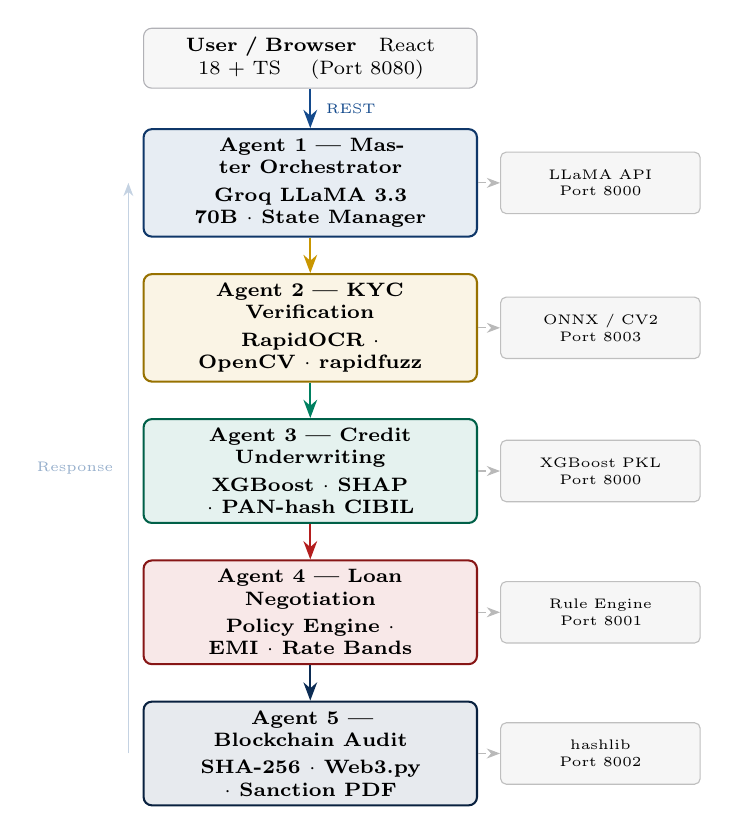
\begin{tikzpicture}[
  font=\scriptsize,
  node distance=0.45cm,
  %% Coloured agent block (1-arg: colour)
  agent/.style={
    rounded corners=3pt,
    draw=#1!75!black,
    fill=#1!10,
    text width=4.0cm,
    minimum height=0.88cm,
    align=center,
    font=\scriptsize\bfseries,
    line width=0.75pt
  },
  %% Small tech tag on right
  tag/.style={
    rounded corners=2pt,
    draw=gray!50,
    fill=gray!7,
    text width=2.3cm,
    minimum height=0.78cm,
    align=center,
    font=\tiny
  },
  %% User / Browser box at top
  userbox/.style={
    rounded corners=3pt,
    draw=loanGray!50,
    fill=gray!6,
    text width=4.0cm,
    minimum height=0.65cm,
    align=center,
    font=\scriptsize
  },
  arr/.style= {-Stealth, thick, #1},
  darr/.style={-Stealth, dashed, thin, gray!55}
]

%% ---- Nodes (vertical chain) ----
\node[userbox] (user)
  {\textbf{User / Browser}\quad React 18 + TS \quad (Port 8080)};

\node[agent=loanBlue, below=0.5cm of user] (orch)
  {\textbf{Agent 1 --- Master Orchestrator}\\[2pt]
   Groq LLaMA 3.3 70B $\cdot$ State Manager};

\node[agent=loanGold, below=of orch] (kyc)
  {\textbf{Agent 2 --- KYC Verification}\\[2pt]
   RapidOCR $\cdot$ OpenCV $\cdot$ rapidfuzz};

\node[agent=loanGreen, below=of kyc] (credit)
  {\textbf{Agent 3 --- Credit Underwriting}\\[2pt]
   XGBoost $\cdot$ SHAP $\cdot$ PAN-hash CIBIL};

\node[agent=loanRed, below=of credit] (neg)
  {\textbf{Agent 4 --- Loan Negotiation}\\[2pt]
   Policy Engine $\cdot$ EMI $\cdot$ Rate Bands};

\node[agent=loanBlue!60!black, below=of neg] (audit)
  {\textbf{Agent 5 --- Blockchain Audit}\\[2pt]
   SHA-256 $\cdot$ Web3.py $\cdot$ Sanction PDF};

%% ---- Tech tags (right side) ----
\node[tag, right=0.28cm of orch]   (t1) {LLaMA API\\Port 8000};
\node[tag, right=0.28cm of kyc]    (t2) {ONNX / CV2\\Port 8003};
\node[tag, right=0.28cm of credit] (t3) {XGBoost PKL\\Port 8000};
\node[tag, right=0.28cm of neg]    (t4) {Rule Engine\\Port 8001};
\node[tag, right=0.28cm of audit]  (t5) {hashlib\\Port 8002};

%% ---- Vertical flow arrows ----
\draw[arr=loanBlue]              (user.south)   -- (orch.north)
  node[midway, right=2pt, font=\tiny]{REST};
\draw[arr=loanGold]              (orch.south)   -- (kyc.north);
\draw[arr=loanGreen]             (kyc.south)    -- (credit.north);
\draw[arr=loanRed]               (credit.south) -- (neg.north);
\draw[arr=loanBlue!60!black]     (neg.south)    -- (audit.north);

%% ---- Tag connectors ----
\draw[darr] (orch.east)   -- (t1.west);
\draw[darr] (kyc.east)    -- (t2.west);
\draw[darr] (credit.east) -- (t3.west);
\draw[darr] (neg.east)    -- (t4.west);
\draw[darr] (audit.east)  -- (t5.west);

%% ---- Return arrow (left spine) ----
\draw[-Stealth, loanBlue!25, thin]
  ([xshift=-0.18cm]audit.west)
  -- ++(0,0)
  -- ([xshift=-0.18cm]orch.west)
  node[midway, left=2pt, font=\tiny, loanBlue!45]{Response};

\end{tikzpicture}
\caption{LoanEase five-agent sequential pipeline. Agents
are invoked in order by the Orchestrator; the left spine
carries the aggregated response back up the chain.}
\label{fig:arch}
\end{figure}

\subsection{Agent 1 — Master Orchestrator Agent}

The Orchestrator is the cognitive center of LoanEase.
Powered by Groq LLaMA 3.3 70B accessed via the Groq
Cloud API, it maintains a persistent conversation state
spanning the full loan lifecycle: identity verification,
credit assessment, offer generation, negotiation, and
sanction. The agent detects user language (English,
Hindi, or Hinglish) via Unicode range analysis and
LLaMA intent classification, then routes each user turn
to the appropriate specialized agent. A structured
system prompt constrains financial terminology (EMI,
KYC, PAN) to remain untranslated, ensuring regulatory
compliance across languages.

\subsection{Agent 2 — KYC Verification Agent}

The KYC Agent processes uploaded PAN card and Aadhaar
card images through a four-stage pipeline: image
preprocessing (CLAHE contrast enhancement, Gaussian
denoising, adaptive thresholding, deskewing via Hough
transform), optical character recognition with
RapidOCR (ONNX-based inference), regex Named Entity
Recognition for field extraction, and rapidfuzz
cross-document name/date-of-birth validation with an
85\% similarity threshold. It exposes four REST
endpoints on port 8003 and returns a structured KYC
status payload with extracted applicant profile and
age eligibility flag.

\subsection{Agent 3 — Credit Underwriting Agent}

The Underwriting Agent performs two-stage credit
evaluation. First, it derives a deterministic simulated
CIBIL score from the SHA-256 hash of the applicant's
PAN number, mapped to the 300--900 range. Second, an
XGBoost classifier trained on the Kaggle Loan
Prediction Dataset computes an approval probability
from 12 financial features. These signals are combined
into a composite risk score, described in
Section~\ref{sec:credit}. SHAP TreeExplainer generates
per-feature contribution values that are translated
into plain-English explanations for the applicant.

\subsection{Agent 4 — Loan Recommendation and
Negotiation Agent}

The Negotiation Agent implements a stateful rule-based
policy engine. Once the Underwriting Agent assigns a
risk tier, the Negotiation Agent initializes a session
with a tier-appropriate starting interest rate,
maximum concession rounds, and a system-wide floor
rate of 10.5\% p.a. The agent decrements the offered
rate by 0.25\% per approved concession round, capping
concessions based on the applicant's credit band, as
detailed in Table~\ref{tab:ratebands}. Sessions expire
after 48 hours. If the floor rate is reached, the agent
escalates the case to a human loan officer.

\subsection{Agent 5 — Blockchain Audit Agent}

Upon loan acceptance, the Blockchain Audit Agent
generates a digitally structured sanction letter,
computes its SHA-256 hash using Python's \texttt{hashlib}
library, and stores the hash with a UTC timestamp and
applicant identifier in a mock distributed ledger
(Ethereum-compatible structure via Web3.py). This
enables tamper verification: any post-generation
modification of the sanction letter changes the hash,
invalidating the on-chain record. The agent is deployed
on port 8002 alongside the translation service.

% ============================================================
%  IV. METHODOLOGY
% ============================================================
\section{Methodology}
\label{sec:methodology}

\subsection{KYC Document Processing Pipeline}

The KYC pipeline ingests uploaded PAN card and Aadhaar
card images (JPEG, PNG, or PDF) through a four-stage
preprocessing chain before OCR extraction. Image
enhancement begins with CLAHE (Contrast Limited
Adaptive Histogram Equalization) applied on the
luminance channel in LAB color space to correct uneven
illumination. Gaussian blur ($\sigma = 1.0$, kernel
$5 \times 5$) reduces high-frequency noise. Adaptive
thresholding (block size 11, constant 2) binarizes the
image. Deskewing is performed via Hough line transform
to detect the predominant text angle and rotate the
image accordingly.

Post-preprocessing, RapidOCR (ONNX-based, CPU inference,
no GPU dependency) performs text detection and
recognition in a two-stage pipeline: a detection model
identifies bounding boxes, and a recognition model
extracts character sequences. Regex-based NER then
isolates structured fields: PAN number
(\texttt{[A-Z]{5}[0-9]{4}[A-Z]}), Aadhaar number
(\texttt{[0-9]{4} [0-9]{4} [0-9]{4}}), full name,
date of birth, and address. Cross-document name/DOB
matching uses rapidfuzz Levenshtein similarity with a
configured threshold of 85\%, tolerating minor OCR
transcription errors. The pipeline is described concisely
in Fig.~\ref{fig:kyc}.

\begin{figure}[!ht]
\centering
\begin{tikzpicture}[
  font=\scriptsize,
  node distance=0.35cm,
  block/.style={
    rounded corners=3pt,
    draw=loanBlue!60,
    fill=loanLightBlue,
    text width=3.8cm,
    minimum height=0.65cm,
    align=center,
    font=\scriptsize
  },
  decision/.style={
    diamond,
    draw=loanGold!80,
    fill=loanLightGold,
    text width=1.8cm,
    minimum height=0.6cm,
    align=center,
    font=\scriptsize,
    inner sep=1pt
  },
  arrow/.style={-Stealth, thick, loanBlue!70}
]

\node[block] (upload) {Document Upload\\(PAN + Aadhaar)};
\node[block, below=of upload] (preproc)
  {Preprocessing\\CLAHE · Gaussian · Threshold · Deskew};
\node[block, below=of preproc] (ocr)
  {RapidOCR Extraction\\(ONNX, CPU Inference)};
\node[block, below=of ocr] (regex)
  {Regex NER\\PAN · Aadhaar · DOB · Name};
\node[decision, below=0.5cm of regex] (match)
  {rapidfuzz\\$\geq$ 85\%?};
\node[block, below=0.5cm of match,
  fill=loanLightGreen, draw=loanGreen!60] (pass)
  {KYC PASS\\Applicant Profile Created};
\node[block, right=1.0cm of match,
  fill=loanLightRed, draw=loanRed!60,
  text width=2.0cm] (fail)
  {KYC FAIL\\Retry Request};

\draw[arrow] (upload) -- (preproc);
\draw[arrow] (preproc) -- (ocr);
\draw[arrow] (ocr) -- (regex);
\draw[arrow] (regex) -- (match);
\draw[arrow] (match) -- node[right=1pt]{Yes} (pass);
\draw[arrow] (match) -- node[above=1pt]{No} (fail);

\end{tikzpicture}
\caption{KYC document processing pipeline. Preprocessing
ensures robust OCR on low-quality scans; rapidfuzz
cross-validation prevents identity spoofing.}
\label{fig:kyc}
\end{figure}

\subsection{Credit Scoring and Underwriting Model}
\label{sec:credit}

\subsubsection{Dataset and Preprocessing}

The model is trained on the publicly available Kaggle
Loan Prediction Dataset containing 614 samples and
12 features: \textit{Gender}, \textit{Married},
\textit{Dependents}, \textit{Education},
\textit{Self\_Employed}, \textit{ApplicantIncome},
\textit{CoapplicantIncome}, \textit{LoanAmount},
\textit{Loan\_Amount\_Term}, \textit{Credit\_History},
\textit{Property\_Area}, and the binary target
\textit{Loan\_Status}. Missing numeric values are
imputed with feature medians; missing categorical
values with per-feature modes. All categorical
features are label-encoded. The dataset is split
80/20 (train/test) with stratified sampling on
\textit{Loan\_Status} to preserve class balance.

\subsubsection{XGBoost Classifier and Hyperparameter Tuning}

An XGBoost binary classifier with \texttt{binary:logistic}
objective is tuned via 5-fold GridSearchCV over the
parameter grid: \texttt{max\_depth} $\in \{3, 4, 5\}$,
\texttt{n\_estimators} $\in \{100, 200\}$, and
\texttt{learning\_rate} $\in \{0.05, 0.1, 0.2\}$,
yielding 18 candidate configurations. The best
configuration is selected on mean cross-validation
accuracy.

\subsubsection{Combined Scoring Formula}

The final composite risk score integrates the simulated
CIBIL credit score and XGBoost approval probability
under a 60/40 weighting:

\begin{equation}
S_{\text{final}} = \left(\frac{C_{\text{CIBIL}} - 300}{600}
  \times 100\right) \times 0.60
  + \left(P_{\text{XGB}} \times 100\right) \times 0.40
\label{eq:score}
\end{equation}

\noindent where $C_{\text{CIBIL}} \in [300, 900]$ is the
simulated bureau score derived deterministically by mapping
the SHA-256 hash of the PAN string to a 300--900 integer
range ($\text{score} = 300 + (\text{hash}_{16} \bmod 601)$),
and $P_{\text{XGB}} \in [0, 1]$ is the XGBoost approval
probability. The resulting $S_{\text{final}} \in [0, 100]$
is then classified into risk tiers that govern interest
rate bands and negotiation rounds (Table~\ref{tab:ratebands}).

\subsubsection{SHAP Explainability}

SHAP TreeExplainer computes exact Shapley values for
every test prediction in $\mathcal{O}(TLD)$ time, where
$T$ is tree count, $L$ is max leaves, and $D$ is feature
count. Feature importances are sorted by absolute mean
SHAP value; the top positive and negative contributors
are translated into plain-English sentences displayed
to the applicant (e.g., \textit{``Your credit history
strongly supports your application.''}).

\subsection{Negotiation Policy Engine}

Table~\ref{tab:ratebands} summarizes the risk-tier-to-rate-band
mapping implemented in the Negotiation Agent.

\begin{table}[H]
\centering
\caption{Risk Tier, CIBIL Band, Interest Rate Range,
and Negotiation Rounds}
\label{tab:ratebands}
\renewcommand{\arraystretch}{1.15}
\begin{tabular}{@{}lcccc@{}}
\toprule
\textbf{Risk Tier} & \textbf{CIBIL} & \textbf{Rate (\%)} &
\textbf{Rounds} & \textbf{Step} \\
\midrule
Low Risk    & 750--900 & 10.5--11.5 & 3 & 0.25\% \\
Low-Medium  & 700--749 & 11.5--12.0 & 2 & 0.25\% \\
Medium Risk & 550--699 & 12.0--13.0 & 1 & 0.25\% \\
High Risk   & 300--549 & 13.5--14.0 & 0 & Fixed  \\
Hard Reject & $<$300   & ---        & 0 & Rejected \\
\bottomrule
\end{tabular}
\end{table}

\noindent The policy engine state machine accepts
\{risk\_tier, rounds\_completed, concessions\_given,
current\_rate, floor\_rate\} and outputs a revised
offer or escalation signal. EMI is computed using the
standard reducing-balance formula:

\begin{equation}
\text{EMI} = \frac{P \cdot R \cdot (1+R)^{N}}{(1+R)^{N}-1}
\label{eq:emi}
\end{equation}

\noindent where $P$ is the principal, $R = r/12/100$
is the monthly interest rate, and $N$ is the tenure
in months. When the floor rate (10.5\% p.a.) is
reached, the session triggers escalation to a human
loan officer rather than issuing a hard rejection.

\subsection{Multilingual Support}

Groq LLaMA 3.3 70B provides context-aware responses
in English, Hindi (Devanagari script), and Hinglish
(romanized Hindi). The translation backend (port 8002)
exposes three endpoints: \texttt{/translate},
\texttt{/detect-hinglish-intent}, and \texttt{/health}.
Language detection performs a first-pass Unicode range
check (Devanagari: U+0900--U+097F) followed by
LLaMA intent classification for ambiguous Hinglish inputs.
The Orchestrator's system prompt explicitly restricts
financial acronyms (EMI, PAN, KYC, CIBIL) and Indian
currency notation (\rupee) from translation, preserving
regulatory and domain correctness.

\subsection{Blockchain Audit Trail}

Upon loan acceptance, the Blockchain Audit Agent
constructs a sanction letter object containing the
applicant's (masked) PAN, loan amount, approved
interest rate, tenure, EMI, sanction reference (e.g.,
\texttt{LE-2026-XXXXX}), and UTC timestamp. The
object is serialized to a canonical JSON string and
its SHA-256 digest computed via Python's \texttt{hashlib}:

\begin{lstlisting}[language=Python, caption={SHA-256
blockchain anchor computation}]
import hashlib, json, time

def anchor_letter(letter_data: dict) -> dict:
    canonical = json.dumps(letter_data,
                           sort_keys=True)
    tx_hash = hashlib.sha256(
        canonical.encode('utf-8')
    ).hexdigest()
    return {
        "tx_hash"   : tx_hash,
        "timestamp" : time.time_ns(),
        "applicant" : letter_data["pan_masked"]
    }
\end{lstlisting}

\noindent The resulting transaction record is appended
to an in-memory mock ledger conforming to the
Ethereum transaction schema (from, to, data, hash,
blockNumber). Verification consists of recomputing the
SHA-256 hash of the stored letter and comparing it
against the ledger entry: a one-bit modification
produces a fully different digest, making tampering
immediately detectable.

% ============================================================
%  V. RESULTS AND EVALUATION
% ============================================================
\section{Results and Evaluation}
\label{sec:results}

\subsection{Credit Underwriting Model Performance}

The XGBoost classifier, tuned with best parameters
\texttt{max\_depth=4}, \texttt{n\_estimators=200},
\texttt{learning\_rate=0.1}, achieves the metrics
shown in Table~\ref{tab:modelperf} on the held-out
20\% test split (123 samples).

\begin{table}[H]
\centering
\caption{XGBoost Credit Underwriting Model Performance}
\label{tab:modelperf}
\renewcommand{\arraystretch}{1.15}
\begin{tabular}{@{}lc@{}}
\toprule
\textbf{Metric} & \textbf{Value} \\
\midrule
Accuracy        & 82.1\%  \\
Precision       & 84.3\%  \\
Recall          & 88.9\%  \\
F1 Score        & 86.5\%  \\
AUC-ROC         & 0.87    \\
Best CV Score   & 80.4\%  \\
\bottomrule
\end{tabular}
\end{table}

\subsection{Model Comparison}

Table~\ref{tab:modelcomp} benchmarks XGBoost against
alternative classifiers under identical preprocessing
and train/test splits, demonstrating its superiority
in both predictive accuracy and explainability.

\begin{table}[H]
\centering
\caption{Classifier Comparison on Loan Prediction Dataset}
\label{tab:modelcomp}
\renewcommand{\arraystretch}{1.15}
\begin{tabular}{@{}lccl@{}}
\toprule
\textbf{Model} & \textbf{Acc.} & \textbf{F1} &
\textbf{Explainable} \\
\midrule
XGBoost (ours)        & \textbf{82.1\%} & \textbf{86.5\%}
  & Yes (SHAP)   \\
Random Forest         & 79.7\% & 83.1\% & Partial (feature imp.) \\
Logistic Regression   & 77.2\% & 81.4\% & Yes (coefficients) \\
Neural Network (MLP)  & 73.8\% & 78.9\% & No \\
\bottomrule
\end{tabular}
\end{table}

\subsection{SHAP Feature Importance}

Fig.~\ref{fig:shap} shows the mean absolute SHAP
values for the top-6 features on the test set.
\textit{Credit\_History} dominates with a SHAP
contribution of 0.41, followed by
\textit{LoanAmount} (0.18) and
\textit{ApplicantIncome} (0.14). This ranking is
consistent with domain expertise: credit history is
the single strongest predictor of loan default
worldwide.

% ---- SHAP bar chart (TikZ) -- explicit coordinates ----
\begin{figure}[!ht]
\centering
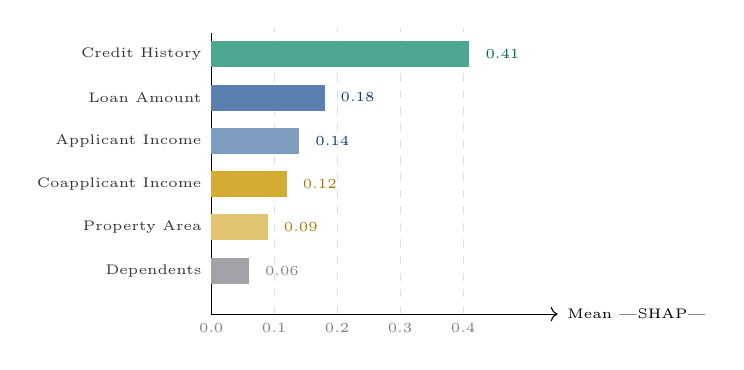
\begin{tikzpicture}[font=\scriptsize, x=8cm, y=0.55cm]

% Axes
\draw[->] (0,0) -- (0.55,0) node[right,font=\tiny] {Mean |SHAP|};
\draw     (0,0) -- (0,6.5);

% Grid lines
\foreach \x in {0.1,0.2,0.3,0.4}
  \draw[gray!25, dashed, thin] (\x,0) -- (\x,6.6);

% X-axis ticks
\foreach \x/\lab in {0/0.0,0.1/0.1,0.2/0.2,0.3/0.3,0.4/0.4}
  \node[below,gray,font=\tiny] at (\x,0) {\lab};

% Bars: {ypos / width / color / label / value-label}
% Row 1 (top)
\fill[loanGreen!70]  (0,5.7) rectangle (0.41,6.3);
\node[right,loanGreen!80!black,font=\tiny] at (0.42,6.0) {0.41};
\node[left, black!80,font=\tiny]            at (0.0, 6.0) {Credit History};

% Row 2
\fill[loanBlue!70]   (0,4.7) rectangle (0.18,5.3);
\node[right,loanBlue!80!black,font=\tiny] at (0.19,5.0) {0.18};
\node[left, black!80,font=\tiny]           at (0.0, 5.0) {Loan Amount};

% Row 3
\fill[loanBlue!55]   (0,3.7) rectangle (0.14,4.3);
\node[right,loanBlue!80!black,font=\tiny] at (0.15,4.0) {0.14};
\node[left, black!80,font=\tiny]           at (0.0, 4.0) {Applicant Income};

% Row 4
\fill[loanGold!80]   (0,2.7) rectangle (0.12,3.3);
\node[right,loanGold!80!black,font=\tiny] at (0.13,3.0) {0.12};
\node[left, black!80,font=\tiny]           at (0.0, 3.0) {Coapplicant Income};

% Row 5
\fill[loanGold!55]   (0,1.7) rectangle (0.09,2.3);
\node[right,loanGold!80!black,font=\tiny] at (0.10,2.0) {0.09};
\node[left, black!80,font=\tiny]           at (0.0, 2.0) {Property Area};

% Row 6
\fill[loanGray!60]   (0,0.7) rectangle (0.06,1.3);
\node[right,loanGray!80,font=\tiny]       at (0.07,1.0) {0.06};
\node[left, black!80,font=\tiny]           at (0.0, 1.0) {Dependents};

\end{tikzpicture}
\caption{Mean absolute SHAP values for top-6 features.
Credit History dominates, confirming domain knowledge.}
\label{fig:shap}
\end{figure}

\subsection{Processing Time Comparison}

Table~\ref{tab:proctime} compares LoanEase's end-to-end
processing time against traditional loan acquisition
channels. LoanEase achieves a \textbf{99.4\% reduction}
in wall-clock processing time compared to the fastest
traditional alternative (bank portal, 2--3 days).

\begin{table}[H]
\centering
\caption{Loan Processing Time: LoanEase vs.\ Traditional Channels}
\label{tab:proctime}
\renewcommand{\arraystretch}{1.15}
\begin{tabular}{@{}lcc@{}}
\toprule
\textbf{Channel} & \textbf{Avg.\ Time} & \textbf{24/7?} \\
\midrule
Traditional Branch    & 7--10 days   & No  \\
Bank Website/App      & 2--3 days    & Partial \\
Loan Agent/DSA        & 3--5 days    & No  \\
\textbf{LoanEase (AI)} & \textbf{$<$ 5 minutes} & \textbf{Yes} \\
\bottomrule
\end{tabular}
\end{table}

\subsection{Feature Comparison with Existing Systems}

Table~\ref{tab:featcomp} benchmarks LoanEase's
capabilities against representative existing solutions.

\begin{table}[H]
\centering
\caption{Feature Comparison: LoanEase vs.\ Existing Systems}
\label{tab:featcomp}
\renewcommand{\arraystretch}{1.15}
\resizebox{\columnwidth}{!}{%
\begin{tabular}{@{}lcccc@{}}
\toprule
\textbf{Feature} & \textbf{LoanEase} &
\textbf{Bank Portal} & \textbf{Fintech App} &
\textbf{DSA Agent} \\
\midrule
Conversational AI      & \checkmark & $\times$ & Partial & $\times$ \\
OCR KYC                & \checkmark & $\times$ & Partial & Manual \\
XAI Explanation        & \checkmark & $\times$ & $\times$ & $\times$ \\
Rate Negotiation       & \checkmark & $\times$ & $\times$ & Manual \\
Multilingual           & \checkmark & Partial  & Partial & Partial \\
Blockchain Audit       & \checkmark & $\times$ & $\times$ & $\times$ \\
24/7 Availability      & \checkmark & \checkmark & \checkmark & $\times$ \\
\bottomrule
\end{tabular}
}
\end{table}

% ============================================================
%  VI. DISCUSSION
% ============================================================
\section{Discussion}

\subsection{Model Selection Rationale}

XGBoost outperforms all evaluated alternatives on this
dataset for several reasons. Gradient boosting
sequentially corrects residual errors of prior
estimators, achieving strong generalization on small,
imbalanced tabular datasets without requiring feature
scaling. Unlike neural networks, XGBoost handles
missing values natively during inference and admits
exact Shapley value computation via TreeExplainer,
which is computationally intractable for deep
architectures. Random forests, while comparable by
accuracy, provide only feature importance rankings
rather than per-prediction attributions, making them
less suitable for regulatory explainability
requirements under RBI guidelines.

\subsection{System Limitations}

Several limitations of the current prototype should be
acknowledged. First, the credit score is simulated via
SHA-256 hash mapping rather than integrated with the
CIBIL TransUnion API, which means the system does not
reflect real credit bureau data in production deployments.
Second, the negotiation engine uses a deterministic
rule-based policy rather than a reinforcement learning
agent, which cannot dynamically adapt concession
strategies based on applicant retention signals.
Third, the XGBoost model is trained on a relatively
small dataset of 614 samples; performance on larger,
more diverse Indian lending datasets (which are
proprietary) remains unvalidated. Finally, the
blockchain component uses a mock in-memory ledger
for the prototype; live Ethereum deployment would
require gas fee management and network latency
considerations.

\subsection{Ethical Considerations}

LoanEase incorporates several design choices aimed at
responsible AI lending. SHAP-based explanations reduce
algorithmic opacity: applicants who receive adverse
decisions are shown the specific features that drove
the outcome, enabling them to understand and
potentially improve their profile. Hard rejections
are accompanied by actionable improvement tips (e.g.,
``Clear outstanding credit card dues,'' ``Maintain
credit utilization below 30\%'') rather than
opaque denials, aligning with the principle of
\textit{contestable} AI decisions \cite{zheng2024blockchain}.
PAN numbers are masked to \texttt{ABCDE****F} format
in all API responses and logs, preventing unintended
PII leakage. The system enforces human escalation
when automated negotiation reaches its floor, ensuring
human oversight remains in the decision loop for
boundary cases.

% ============================================================
%  VII. CONCLUSION AND FUTURE WORK
% ============================================================
\section{Conclusion and Future Work}

This paper has presented LoanEase, a multi-agent AI
system that automates the complete personal loan
lifecycle through five collaborating FastAPI
microservices orchestrated by a Groq LLaMA 3.3 70B
master agent. The system achieves a 99.4\% reduction
in loan processing time compared to traditional
bank branches, while providing OCR-based KYC
verification, XGBoost underwriting with SHAP
explainability, multi-round interest rate negotiation
bounded by risk-tier policy, multilingual Hindi and
English conversational support, and SHA-256 blockchain
anchor for sanction letter auditability. The XGBoost
model achieves 82.1\% accuracy and an AUC-ROC of 0.87
on the Kaggle Loan Prediction Dataset, outperforming
Random Forest, Logistic Regression, and MLP baselines.

Future work will address the limitations identified
above through several research directions. The
simulated credit score module will be replaced with a
live integration to the CIBIL TransUnion API or CRIF
High Mark bureau upon obtaining regulatory authorization,
enabling production-grade underwriting. The rule-based
negotiation engine will be replaced by a deep
reinforcement learning agent trained to maximize
loan acceptance rate subject to bank margin constraints,
dynamically adapting to applicant negotiation behavior.
The training dataset will be expanded using proprietary
Indian NBFC lending records under data-sharing agreements.
The mock blockchain will be migrated to a live Ethereum
or Polygon deployment with on-chain smart contract
verification. The system will be extended to cover home
loans, gold loans, and MSME business loans with
product-specific underwriting models. Regulatory
compliance with RBI's Digital Lending Guidelines (2022)
and the Payment Aggregator Framework will be fully
implemented. A voice interface using Whisper ASR and
TTS will be added to serve rural and low-literacy
applicants who cannot engage with a text-based chat
interface, directly addressing the digital divide in
Indian financial inclusion.

% ============================================================
%  ACKNOWLEDGMENT
% ============================================================
\section*{Acknowledgment}

The authors thank Dr.\ Mansi Kambli, Department of
Computer Engineering, K.J.\ Somaiya College of
Engineering, for her patient guidance and invaluable
domain expertise throughout this project. We also
acknowledge the open-source communities behind
XGBoost, SHAP, RapidOCR, FastAPI, and Groq for
making this research reproducible.

% ============================================================
%  REFERENCES
% ============================================================
\bibliographystyle{IEEEtran}

\begin{thebibliography}{15}

\bibitem{wu2023autogen}
Q.\ Wu, G.\ Bansal, J.\ Zhang, et al., ``AutoGen: Enabling
Next-Gen LLM Applications via Multi-Agent Conversation,''
\textit{arXiv preprint arXiv:2308.08155}, 2023.

\bibitem{park2023generative}
J.\ S.\ Park, J.\ C.\ O'Brien, C.\ J.\ Cai, M.\ R.\ Morris,
P.\ Liang, and M.\ S.\ Bernstein, ``Generative Agents:
Interactive Simulacra of Human Behavior,''
\textit{arXiv preprint arXiv:2304.03442}, 2023.

\bibitem{soleh2024creditxai}
A.\ Soleh and R.\ Tamura, ``CreditXAI: Explainable Credit
Scoring Using Transformer Embeddings and SHAP Attribution,''
\textit{arXiv preprint arXiv:2510.22222}, 2024.

\bibitem{hazra2025agentic}
A.\ Hazra, S.\ Sharma, and P.\ Gupta, ``Agentic AI for
Credit Risk: Autonomous Assessment Pipelines Using Large
Language Models,'' \textit{arXiv preprint arXiv:2601.00818},
2025.

\bibitem{tripathi2023ml}
R.\ Tripathi, S.\ Verma, and N.\ Mehta, ``A Systematic
Review of Machine Learning Methods for Credit Risk
Assessment,'' \textit{Risks}, MDPI, vol.\ 11, no.\ 9,
p.\ 161, 2023.

\bibitem{autogen2025}
Microsoft Research, ``AutoGen: Multi-Agent Conversation
Framework for Complex LLM Applications,''
\textit{Technical Report}, Microsoft, 2025.
[Online]. Available: \url{https://microsoft.github.io/autogen/}

\bibitem{wang2024survey}
L.\ Wang, C.\ Ma, X.\ Feng, et al., ``A Survey on Large
Language Model-Based Autonomous Agents,''
\textit{arXiv preprint arXiv:2401.13488}, 2024.

\bibitem{zheng2024blockchain}
Y.\ Zheng, H.\ Xie, T.\ Dai, C.\ Chen, and H.\ Wang,
``Blockchain Applications in Financial Accounting and
Reporting: A Systematic Review,''
\textit{Journal of Risk and Financial Management}, MDPI,
vol.\ 17, no.\ 2, pp.\ 1--24, 2024.

\bibitem{chen2016xgboost}
T.\ Chen and C.\ Guestrin, ``XGBoost: A Scalable Tree
Boosting System,'' in \textit{Proc.\ 22nd ACM SIGKDD
Int.\ Conf.\ Knowledge Discovery and Data Mining (KDD)},
pp.\ 785--794, 2016.

\bibitem{groq2024llama}
Groq Inc., ``Groq LPU Inference Engine and LLaMA 3.3 70B
API Reference,'' Technical Documentation, 2024.
[Online]. Available: \url{https://console.groq.com/docs/}

\bibitem{rbi2024}
Reserve Bank of India, ``Report on Trend and Progress of
Banking in India 2023--24,'' RBI Publications, 2024.
[Online]. Available: \url{https://www.rbi.org.in}

\bibitem{niti2023digitalfinance}
NITI Aayog, ``India's Booming Digital Lending: A
Regulation Focus,'' Government of India, 2023.

\bibitem{lundberg2017shap}
S.\ M.\ Lundberg and S.-I.\ Lee, ``A Unified Approach to
Interpreting Model Predictions,'' in \textit{Advances in
Neural Information Processing Systems (NeurIPS)},
vol.\ 30, 2017.

\bibitem{rapidocr2023}
RapidAI, ``RapidOCR: A Practical Ultra-Lightweight
ONNX-Based OCR Tool,'' GitHub Repository, 2023.
[Online]. Available: \url{https://github.com/RapidAI/RapidOCR}

\bibitem{kaggle2023loan}
Analytics Vidhya, ``Loan Prediction Problem Dataset,''
\textit{Kaggle}, 2023.
[Online]. Available: \url{https://www.kaggle.com/datasets/altruistdelhite04/loan-prediction-problem-dataset}

\end{thebibliography}

\end{document}
